\section[A simple example: MLP]{A simple example: classify handwritten digits with a \acl{MLP}}

\begin{frame}
  \note{
    \begin{itemize}
    \item Explain why we will talk about the MLP
    \item Rosenblatt was NOT at Dartmouth conference but his research was
      founded as part of the beginning of AI
    \end{itemize}
  }

  \frametitle{\acl{MLP}: Introduction}

  \begin{textblock}{55}(5, 15)
    \begin{itemize}
    \item<1-> First perceptron was introduced in 1957 by Frank Rosenblatt:
      \begin{itemize}
      \item One of the first \acl{NN}
      \item Loose biological inspiration
      \item No hidden layers, no activation function
      \item No learning
      \end{itemize}
    \item<2-> Many improvements since then:
      \begin{itemize}
      \item Hidden layers and activation functions $\rightarrow$ \ac{MLP}
      \item Lots of variations
      \end{itemize}
    \item<3-> The \ac{MLP} is one of the most studied architecture
    \end{itemize}
  \end{textblock}

  \begin{textblock}{30}(70, 10)
    \begin{center}
      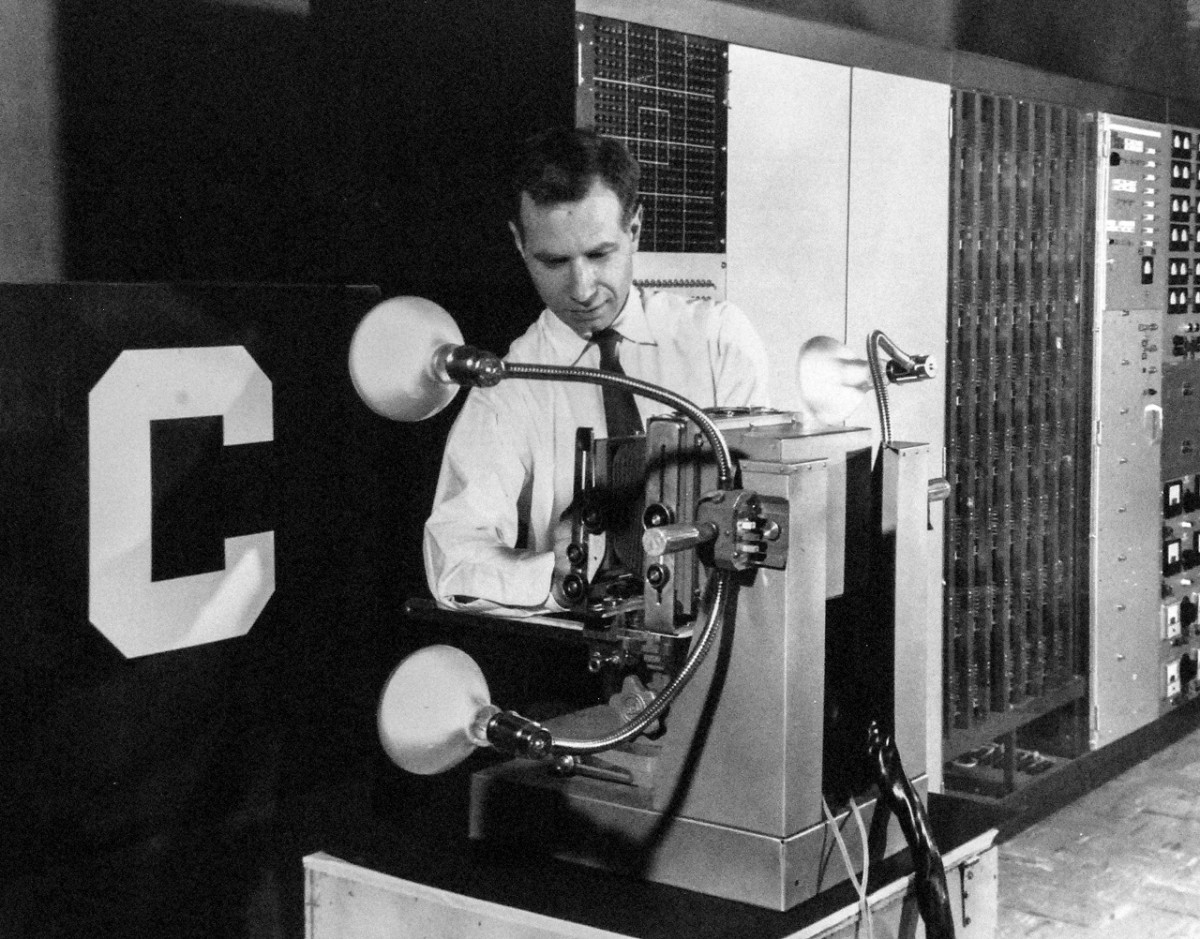
\includegraphics[width=\textwidth]{img/MLP.jpg}
      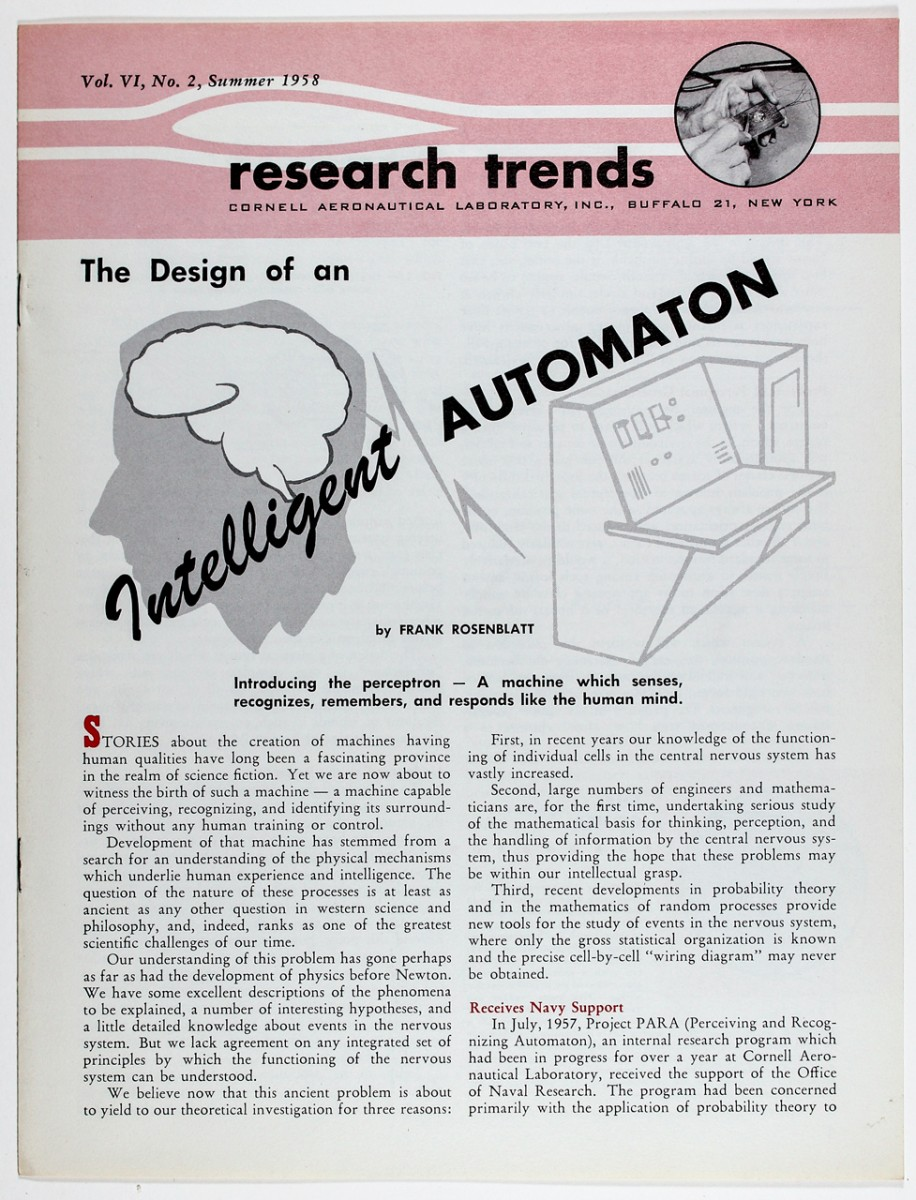
\includegraphics[width=\textwidth]{img/MLP_Cover.jpg}
    \end{center}
  \end{textblock}
\end{frame}


\subsection{How does it work?}

\begin{frame}
  \note{
    \begin{itemize}
    \item Don't forget to talk about neurons :)
    \item Probabilistic classifier:
      \begin{align*}
        \begin{aligned}
          & \hyp_{\params} : & \setR^{\dimExample} & \rightarrow & \interval{0}{1}^{\nClasses} \\
        \end{aligned}
      \end{align*}
      where
      $\vector{\predLabel} = \apply{\hyp_{\params}}{\example}$ is a vector such
      that $\vectorElem{\vector{\predLabel}}{k}$ is $\prob{\example = k}$
    \item Feed-forward
    \item Parametrized function
    \item Importance of non-linear activation function
    \item Note that we neglected bias term
    \item Idea:
      \begin{itemize}
      \item Hidden layers learn internal representations of the data
      \end{itemize}
    \end{itemize}
  }

  \frametitle{\acl{MLP}: Computation}
  \begin{textblock}{100}(5,15)
    \begin{tikzpicture}[>=stealth]
      % Inspired by https://tex.stackexchange.com/a/153974
      % We display a MLP with 2 hidden layers for OCR
      % The input image and the output layer are always displayed
      % The layers (input and the 2 hidden) and their connections appear after
      % Description of layers are on the graph
      % The number of neurons per layer is taken from
      % Gradient-Based Learning Applied to Document Recognition, Le Cun et al., 1998

      % Parameters
      \def\xInputImage{0}
      \def\nameInputImage{input-name}
      \def\xInput{2.0}
      \def\nameInput{input}
      \def\xHiddenI{4.3}
      \def\nameHiddenI{hidden1}
      \def\xHiddenII{6.6}
      \def\nameHiddenII{hidden2}
      \def\xOutput{8.9}
      \def\nameOutput{output}
      \def\xProba{9.4}
      \def\nameProba{proba}
      \def\missing{missing}

      % Input image and grid
      % This part is inspired by https://tex.stackexchange.com/a/128648
      % and a lot of trial and error for the grid (including a bit of ChatGPT)
      % Apparently, the idea is to fix the size of the image and then the grid
      % flows
      % I use 56px (twice the real size) so that it looks OK and computations are easy.
      \node[anchor=center,inner sep=0pt,draw=black] (\nameInputImage) at (\xInputImage,0) {
        
\includegraphics[width=56px,height=56px]{img/Mnist_8.png}
      };
      \begin{scope}
        \clip (\nameInputImage.south west) rectangle (\nameInputImage.north east);
        \draw[step=2px,gray,very thin] (\nameInputImage.south west) grid (56px, 56px);
      \end{scope}

      \onslide<2->{
      % Input layer
      \node [align=center, above] at (\xInput,2.2) {%Input \\ layer \\
          {\tiny $28\times28=784$ units}};
      \foreach \m/\l [count=\y] in {1,2,3,missing,784}
      \node [every neuron/.try, neuron \m/.try] (\nameInput-\m) at (\xInput,3.0-\y) {};

      % Connections from input image to input layer
      % No loop here cause we need to shift the positions
      % It uses the scale introduced above
      \draw [->] (\nameInputImage)++(-27px,27px) -- (\nameInput-1);
      \draw [->] (\nameInputImage)++(-25px,27px) -- (\nameInput-2);
      \draw [->] (\nameInputImage)++(-23px,27px) -- (\nameInput-3);
      \draw [->] (\nameInputImage)++(27px,-27px) -- (\nameInput-784);
      }

      % Description of the output
      \onslide<2>{
      \node[text width=3cm,anchor=north west] at (\xInput-1, -2.2) {{\footnotesize
          $\output^{1}_{k} = \vectorElem{\example}{k}$
      }} ;
      }

      % Matrix form
      \onslide<3->{
      \node[text width=3cm,anchor=north west] at (\xInput-1, -2.2) {{\footnotesize
          $\vector{\output}^{1} = \example$
      }} ;
      }

      % First hidden layer
      % Connections are displayed in 2 different slides (see below)
      \onslide<3->{
      \node [align=center, above] at (\xHiddenI,2.2) {%Hidden \\ layer \\
          {\tiny 300 $\ReLUFunc$ units}};
      \foreach \m [count=\y] in {1,2,missing,3}
      \node [every neuron/.try, neuron \m/.try ] (\nameHiddenI-\m) at (\xHiddenI,2.5-\y) {};
      }

      % Connections from input layer to first neuron with weights
      % and explanation of the output
      \onslide<3>{
      \foreach \p in {1,2,3,784}
      \foreach \k in {1}
      \draw[->] (\nameInput-\p) -- node {${\color{red} \weight^{1}_{\k,\p}}$} (\nameHiddenI-\k);

      % Description of the output
      \node[text width=3cm,anchor=north west] at (\xHiddenI-1, -2.2) {{\footnotesize
          $s^{2}_{k} = \sum_{p=1}^{N_{1}} {\color{red} \weight^{1}_{k,p}} \output^{1}_{p} $
      }};
      \node[text width=5cm,anchor=north west] at (\xHiddenI-1, -3.0) {{\footnotesize
          $\output^{2}_{k} = \apply{\ReLUFuncExt}{0, s^{2}_{k}}$ ($\ReLUFunc$)
      }};
      }

      % Other connections from input layer to first hidden layer
      % and matrix form
      \onslide<4->{
      \foreach \i in {1,2,3,784}
      \foreach \j in {1,...,3}
      \draw[->] (\nameInput-\i) -- (\nameHiddenI-\j);
      \node[text width=3cm,anchor=north west] at (\xHiddenI-1.2, -2.2) {{\footnotesize
          $\vector{\output^{2}} = \apply{\ReLUFunc}{{\color{red}\weightMatrix^{1}}\vector{\output^{1}}}$
      }};
      }

      % Second hidden layer
      \onslide<5->{
      \node [align=center, above] at (\xHiddenII,2.2) {% Hidden \\ layer \\
          {\tiny 100 $\ReLUFunc$ units}};
      \foreach \m [count=\y] in {1,2,missing,3}
      \node [every neuron/.try, neuron \m/.try ] (\nameHiddenII-\m) at (\xHiddenII,2.2-0.9*\y) {};

      % Connections to first hidden layer to second hidden layer
      \foreach \i in {1,2,3}
      \foreach \j in {1,2,3}
      \draw [->] (\nameHiddenI-\i) -- (\nameHiddenII-\j);

      \node[text width=3cm,anchor=north west] at (\xHiddenII-1, -2.4) {{\footnotesize
          $\vector{\output^{3}} = \apply{\ReLUFunc}{{\color{red}\weightMatrix^{2}}\vector{\output^{2}}}$
      }};
      }

      % Output layer
      \node [align=center, above] at (\xOutput,2.2) {% Output \\ layer \\
        {\tiny 10 $\softMaxFunc$ units}};
      \foreach \m [count=\y] in {0,1,missing,9}
      \node [every neuron/.try, neuron \m/.try ] (\nameOutput-\m) at (\xOutput,1.6-0.7*\y) {};

      \onslide<6->{
      % Connection from second hidden layer to output layer
      \foreach \i in {1,2,3}
      \foreach \j in {0,1,9}
      \draw [->] (\nameHiddenII-\i) -- (\nameOutput-\j);
      }

      % Description of output
      \onslide<6>{
      \node[text width=3cm,anchor=north west] at (\xOutput-0.5, -2.2) {{\footnotesize
          $s^{4}_{k} = \sum_{p=1}^{N_{3}} {\color{red} \weight^{3}_{k,p}} \output^{3}_{p}$
      }};
      \node[text width=5cm,anchor=north west] at (\xOutput-0.5, -3.0) {{\footnotesize
          $\output^{4}_{k} = \frac{\apply{\exp}{s^{4}_{k}}}{\sum_{j=1}^{10} \apply{\exp}{s^{4}_{j}}}$
      }};
      }

      \onslide<7->{
      \node[text width=3cm,anchor=north west] at (\xOutput-0.7, -2.2) {{\footnotesize
          $\vector{\output^{4}} = \apply{\softMaxFunc}{{\color{red}\weightMatrix^{3}}\vector{\output^{3}}}$
      }};
      }


      % Output probabilities
      \foreach \m [count=\y] in {0,1,missing,9}
      \node (\nameProba-\m) at (\xProba,1.6-0.7*\y) {\ifx\m\missing\else {\tiny $\prob{\m}$}\fi};

      % Description (put above for clarity)
      \onslide<7->{
      \node[text width=10cm,anchor=north west] at (-1, 3.5) {{\footnotesize
          \acsu{MLP} is a parametrized function $\hyp_{\params}$ where
          ${\color{red}\params}$ is the vector containing the {\tiny $784 \times
          300 + 300 \times 100 + 100 \times 10 = $} 266 200 weights
      }};
      }
    \end{tikzpicture}

  \end{textblock}

\end{frame}


\subsection{Learning}

\begin{frame}
  \frametitle{\acl{MLP}: Learning (1/2)}

  \begin{block}{Goal}
    Adjust $\params$ to give a better performance
  \end{block}

  \begin{block}{General idea}<2->
    %Bad prediction: $\predLabel_i =
    %\apply{\hyp_\params}{\example_i}$ is far from $\knownLabel_i$
    \begin{itemize}
    \item<2-> Define a loss function $\lossFunc$ such that $\apply{\lossFunc}{
            \apply{\hyp_\params}{\example_i},
            \knownLabel_i
          }$ is high if $\apply{\hyp_\params}{\example_i}$ is far from
          $\knownLabel_i$
     \item<3-> Minimize $\lossFunc$ (as a function of $\params$)
     \item<4-> The correct loss function depends on the problem
    \end{itemize}
  \end{block}

  \begin{block}{In our example}<5->
    \begin{itemize}
    \def\vectorextleftdelim{(}
    \def\vectorextrightdelim{)}
    \item $\output_i^4 = \apply{\hyp_\params}{\example_i}$ is a vector $\vectorext{\prob{0}, \prob{1}, \cdots,
        \prob{8}, \prob{9}}^T$
    \item $u_i$ is the label \onslide<6->{$\rightarrow$ transform it $\vectorext{0, 0, \cdots, 1, 0}^T$ (one-hot
      encoding)}
  \item<7-> Cross-entropy loss:
    \begin{center}
      $
        \apply{\lossFunc}{\apply{\hyp_\params}{\example_i},
          \knownLabel_i} = \only<7>{- \sum_{k=1}^{10} \knownLabel_{i,k}
          \apply{\log}{\output_{i,k}^4}}
                           \only<8->{- \apply{\log}{\prob{8}}}
      $
    \end{center}
    \item<9-> Cross-entropy is more general
    \end{itemize}
  \end{block}
\end{frame}


% This frame allows to jump to frames explaining back-propagation (file
% appendix_mlp)
% We come back on slide 6. The algorithm is also adapted on this slide
\begin{frame}
  \note{
    \begin{itemize}
    \item Present the general idea of gradient descent
      \begin{itemize}
      \item Mention epochs
      \end{itemize}
    \item Jump to other frames for details of back-propagation
    \item Come back to conclude:
      \begin{itemize}
      \item We now have a full learning procedures for our MLP
      \item Now you understand why it took almost 30 years :)
      \end{itemize}
    \end{itemize}
  }
  \frametitle{\acl{MLP}: Learning (2/2)}
  % Define the target to come back from the frames explaining backpropagation
  % It's on slide 6 (see below)
  \hypertarget<6>{MLP_Learning_2}{}

  \begin{textblock}{45}(5,15)
    \begin{block}{How to minimize $\lossFunc$?}
      \onslide<2->{
        If we know the gradient of $\lossFunc$ at $\params_{t}$ we can update:
        \[
          \params_{t+1} \leftarrow \params_{t} - \learningRate
          \apply{\grad_{\params}\lossFunc}{\params_{t}}
        \]
      }
    \end{block}
  \end{textblock}

  % Cheat a bit on the position
  \begin{textblock}{50}(50,10)
    \begin{center}
    \begin{tikzpicture}[domain=0:4,yscale=0.8]
      % Display a 1-D analytical loss function (x-2)**2 + 0.3
      % to illustrate
      \def\paramsInit{3} % Current value of the parameter
      \def\lossInit{1.3} % Current value of the loss
      \def\gradVal{2}    % Value of the gradient

      % \draw[very thin,color=gray] (-0.1,-0.1) grid (3.9,3.9);
      \draw[->] (-0.2,0) -- (4.2,0) node[right] {$\params$};
      \draw[->] (0,-0.2) -- (0,4.2) node[above right] {$\apply{\lossFunc}{\apply{\hyp_{\params}}{\example_i}, \knownLabel_i}$};
      % Display loss function
      \draw[color=blue] plot function{(x-2)**2+0.3} node[right] {};

      % Value at \paramsInit
      \node[anchor=north] at (\paramsInit, 0) {$\params_{t}$};
      \draw[dashed] (\paramsInit, 0) -- (\paramsInit, \lossInit) {};

      % Gradient at \paramsInit
      \onslide<2->{
      \draw[->,color=red,thick] (\paramsInit, \lossInit) -- (\paramsInit + 0.5, \lossInit + 0.5*\gradVal) {};
      \node[anchor=west] at (\paramsInit + 0.5, \lossInit + 0.5*\gradVal) {${\color{red}\apply{\grad_{\params}\lossFunc}{\params_{t}}}$};
      }
    \end{tikzpicture}
    \end{center}
  \end{textblock}

  \begin{textblock}{45}(5, 55)
    \onslide<3->{
      \begin{block}{Gradient descent}
        \only<3-5>{
          \begin{algorithm}[H]
            \SetAlgoLined
            \DontPrintSemicolon
            \SetKwFunction{Initialize}{Initialize\_Weights}
            \SetKwFunction{Convergence}{Convergence}
            \SetKwFunction{ComputeGrad}{Compute\_Grad}

            $\params \leftarrow \Initialize()$\;
            \While{$\neg \Convergence()$}{
              \For{$\example_i \in \trainingSet$}{
                $grad \leftarrow \ComputeGrad(\params)$\;
                $\params \leftarrow \params - \learningRate \times grad $\;
              }
            }
            Return $\params$\;
          \end{algorithm}
        }
        \only<6->{
          \begin{algorithm}[H]
            \SetAlgoLined
            \DontPrintSemicolon
            \SetKwFunction{Initialize}{Initialize\_Weights}
            \SetKwFunction{Convergence}{Convergence}
            \SetKwFunction{ComputeGrad}{{\color{red}Back\_Prop}}

            $\params \leftarrow \Initialize()$\;
            \While{$\neg \Convergence()$}{
              \For{$\example_i \in \trainingSet$}{
                $grad \leftarrow \ComputeGrad(\params)$\;
                $\params \leftarrow \params - \learningRate \times grad $\;
              }
            }
            Return $\params$\;
          \end{algorithm}
        }
      \end{block}
    }
  \end{textblock}

  \begin{textblock}{45}(50, 55)
    \onslide<4->{
      \begin{itemize}
      \item Generic algorithm
      \item<5-> We must compute
        $\apply{\grad_{\params}\lossFunc}{\params_{t}}$
        % Display the entry and the "Details" button on slide 5
        % Some text is added on slide 6
      \item<5->
        \only<6->{
          Back-propagation is an efficient method for that in feed-forward
          architectures
        }
        \hyperlink{Backpropagation}{\beamergotobutton{Details}}
        % \item Many practical adjustments:
      %   \begin{itemize}
      %   \item Initialization
      %   \item Mini-batch, shuffling
      %   \item Convergence criteria
      %   \item Smarter minimization algorithm
      %   \end{itemize}
    \end{itemize}
  }
  \end{textblock}
\end{frame}


\begin{frame}
  \note{
    \begin{itemize}
    \item Present hyper-parameter and how to tune them
    \item Insist on the number of variations especially for more complex models
    \end{itemize}
  }
  \frametitle{\acl{MLP}: Hyper-parameters}

  \begin{textblock}{90}(5, 15)
    \begin{block}{Parameters that are not learned:}
      \begin{itemize}
      \item<1-> Architecture variations:
        \begin{itemize}
        \item Number of neurons per hidden layer
        \item Number of hidden layers
        \item Activation functions
        \item Connectivity pattern
        \item \etc{}
        \end{itemize}
      \item<2-> Learning procedure variations:
        \begin{itemize}
        \item Learning rate: value, adaptive, \etc{}
        \item Mini-batches
        \item Initalization
        \end{itemize}
      \end{itemize}
    \end{block}
  \end{textblock}

  \begin{textblock}{90}(5, 70)
    \onslide<3->{
      \begin{block}{How to tune them?}
        \begin{itemize}
        \item Several techniques: grid-search
        \item Need to reserve some data for that
        \end{itemize}
      \end{block}
    }
  \end{textblock}
\end{frame}


\subsection{Results}

\begin{frame}
  \note{
    \begin{itemize}
    \item Importance of evaluation:
      \begin{itemize}
      \item Especially in the face of ethical issues
      \item Teams dedicated to that (Guigui mon amour :)
      \end{itemize}
    \item Results of MLP
    \end{itemize}
  }
  \frametitle{\acl{MLP}: Results and interpretation}

  \begin{textblock}{90}(5, 15)
    \begin{block}{Evaluation metrics}
      \begin{itemize}
      \item Evaluation metrics plays a crucial role in ML
      \item Can be different than the loss function
      \item The metric to use depends on the task
      \end{itemize}
    \end{block}
  \end{textblock}

  \begin{textblock}{90}(5, 40)
    \onslide<2->{
      \begin{block}{In our example}
        \begin{itemize}
        \item The most natural metric is the accuracy (\ie{} correct prediction
          rate) on the test set
        \item \ac{MLP} car reach an error rate of $\approx 3\%$
        \end{itemize}
      \end{block}
    }
  \end{textblock}
\end{frame}


\begin{frame}
  \note{
    \begin{itemize}
    \item Tentative interpretation
    \item Link to \acf{xAI}
    \end{itemize}
  }
  \frametitle{\acl{MLP}: Interpretation}

  % Cheat a bit on the height so figure is larger
  \begin{textblock}{90}(5, 10)
    \begin{block}{Can we understand how does it work?}
      \onslide<2->{
        Plot the first weights:
        \begin{center}
          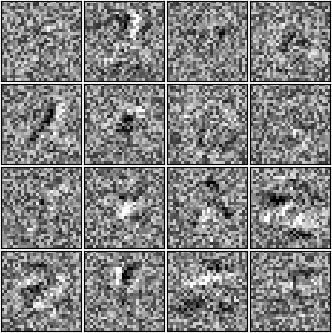
\includegraphics[width=0.5\textwidth]{img/MLP_Weights.png}
        \end{center}
      }
    \end{block}
  \end{textblock}
\end{frame}
